\documentclass{sig-alternate}

\begin{document}

\title{Cheminformatics: The Computer Science of Chemical Discovery}
\numberofauthors{9}
\author{
\alignauthor
Joerg Kurt Wegner\\
       \affaddr{Tibotec BVBA}\\
       \affaddr{Turnhoutseweg 30}\\
       \affaddr{2340 Beerse Turnhout, Belgium}\\
       \email{jwegner@its.jnj.com}
% 2nd. author
\alignauthor
Aaron Sterling\\
       \affaddr{Department of Computer Science}\\
       \affaddr{Iowa State University}\\
       \affaddr{Ames, Iowa, USA}\\
       \email{sterling@iastate.edu}
% 3rd author
\alignauthor
Rajarshi Guha\\
\affaddr{NIH Center for Translational Therapeutics}\\
\affaddr{9800 Medical Center Drive}\\
\affaddr{Rockville, MD 20850}\\
\email{guhar@mail.nih.gov}
}

\additionalauthors{Additional authors:
Andreas Bender (University of Cambridge, email: {\texttt{bender.andreas@gmail.com}}),
Jean-Loup Faulon (University of Evry, email: {\texttt{Jean-Loup.Faulon@issb.genopole.fr}}),
Janna Hastings (European Bioinformatics Institute, Cambridge, UK, email: {\texttt{janna.hastings@gmail.com}}),
Noel O'Boyle (University College Cork, Cork, Ireland, email: {\texttt{baoilleach@gmail.com}}),
John Overington (European Bioinformatics Institute, Cambridge, UK, email: {\texttt{jpo@ebi.ac.uk}}),
Herman Van Vlijmen (Tibotec, Beerse, Belgium, email: {\texttt{hvvlijme@its.jnj.com}}), and
Egon Willighagen (Karolinska Institutet, Stockholm, Sweden, email: {\texttt{egon.willighagen@ki.se}})
.}
\date{25 June 2011}


\maketitle
\begin{abstract}
One of the most prominent success stories in all the sciences over the last decade has
  been the advance of bioinformatics: interdisciplinary collaboration between
 computer scientists and molecular biologists led to the sequencing of the human genome
  and many other accomplishments, since researchers connected biological
  concepts to the theory of string algorithms. However, despite this great
  success, few computer scientists are familiar with a related (and older!)
  discipline---cheminformatics, the use of computers to represent
 the structures of small molecules and analyze their properties.
  Cheminformatics has a wide applicability,
  from the discovery of novel drug candidates to the optimization of
  certain physicochemical properties of small molecules. Until
 recently, the data and techniques of cheminformatics have been closely guarded
  secrets of companies whose financial success depended on being the first to produce
  the new ``miracle molecule.'' Only within the last decade---and largely because of
 chemists volunteering their time for an Open Science ``movement''---have researchers
  gained access to freely available software packages and databases of tens of
  millions of chemicals. Academic chemists now confront a variety of unsolved
  algorithmic problems that could not have been tackled a decade ago, but whose
  solutions are critical to research ranging from determining the behavior of small
  molecules in biological pathways, to finding a cure for malaria.
\end{abstract}

\category{H.4}{Information Systems Applications}{Miscellaneous}
\terms{
\begin{itemize}
\item \textit{Bioassay} - A system measuring the biological activity of a chemical compound on a particular biological assay (with all its parameters).
\item \textit{Biodegradation} - is the chemical dissolution of materials by bacteria or other biological means.
\item \textit{Conformation and conformational isomerism} - In chemistry, conformational isomerism is a form of stereoisomerism in which the isomers can be interconverted exclusively by rotations about formally single bonds. Single possible states of compounds are called conformers.
\item \textit{Ligand (biochemistry)} - a substance that binds to a protein.
\item \textit{Ligand (coordination chemistry)} - an atom, ion, or functional group that donates one or more of its electrons through a coordinate covalent bond to one or more central atoms or ions.
\item \textit{Mass spectrometry} - Mass spectrometry (MS) is an analytical technique that measures the mass-to-charge ratio of charged particles. It is used for determining masses of particles, for determining the elemental composition of a sample or molecule, and for elucidating the chemical structures of molecules, such as peptides and other chemical compounds.
\item \textit{Metabolites} - Metabolites are the intermediates and products of metabolism. The term metabolite is usually restricted to small molecules (chemical compounds).
\item \textit{Proteochemometric modeling} - combining data mining for chemical compounds (ligands) and proteins within the same machine learning framework.
\item \textit{Protonation and protonation state} - In chemistry, protonation is the addition of a proton (H$^+$) to an atom, molecule, or ion. The different states (different number of H$^+$ or on different atoms) are called protonation states for a molecular compound (e.g. de-protonated, mono-protonated, di-protonated, or any variations of those states).
\item \textit{Reaction catalysis} - Catalysis is the change in rate of a chemical reaction due to the participation of a substance called a catalyst.
\item \textit{Receptor (biochemistry)} - in biochemistry, a protein molecule that receives and responds to a neurotransmitter, or other substance.
\item \textit{Regulation authorities} - In the US the Food and Drug Administration (FDA) is responsible for protecting and promoting public health through the regulation and supervision of e.g. dietary supplements, prescription and over-the-counter pharmaceutical drugs (medications), vaccines, biopharmaceuticals, medical devices, and many other health related items. The European Medicines Agency (EMA) is a European agency for the evaluation of medicinal products.
\item \textit{SMARTS} - SMiles ARbitrary Target Specification \\(SMARTS) is a language for specifying substructure patterns in molecules
\item \textit{Stereoisomer/stereoisomerism} - Stereoisomers are isomeric molecules that have the same molecular formula and sequence of bonded atoms (constitution), but that differ only in the three-dimensional orientations of their atoms in space.
\item \textit{Tautomerism} - Tautomers are isomers (same molecular formula but different structural formula) of organic compounds that readily interconvert by a chemical reaction called tautomerization.
\end{itemize}
}
\keywords{cheminformatics, graphs, chemistry, databases, knowledge management, open source, open data}

\section{Is Cheminformatics the New \\Bioinformatics?}

Novel technologies in the life sciences churn out information at an ever
increasing rate---public data stores such as the one at the European Bioinformatics
Institute (EBI) contain on the order of 10 petabytes of biological information.
However, while biological information has been publicly available for decades,
the same has not been true for chemical information until very recently. It was
not until 2004 that a large public small molecule structure repository (PubChem)
became freely available. This was followed by other databases, as discussed later
in this article. In the same vein, open source software and the publication of
algorithms have only recently become a main focus of the field
\cite{faulon2010}.

So why should we actually care about chemical information being made
public---and how does this relate to the field of computer science?

Making chemical information public is important because the
drugs we take are the result of intensive and costly research,
which is facilitated by the extent of information available. The
more information is shared (a process very hard to achieve
in pharmaceutical companies), the more information is available to each
researcher, facilitating the development of
novel treatments. The relevance of computer
science in this research becomes clear in considering the quantity of data available
currently---74 million different molecules are currently stored in
public databases (such as PubChem), together with an even larger number of annotations.
The design of data structures for this chemical information, as well as subsequent
data mining of this information, are areas where expertise in computer
science is urgently needed. (For a recent, detailed introduction to
cheminformatics, written for computer scientists, see
\cite{brown2009}).

Cheminformatics comprises different areas, which broadly speaking can be divided
into three fields: \emph{capturing data} (using lab notebooks or potentially using
formats such as the Chemical Markup Language for publications); \emph{storing data}
(designing database schemas, devising ontologies) and \emph{mining data} (such as for
bioactivity prediction, which might involve algorithms based on graphs).
However, a major difference from bioinformatics lies in the type of
information being analyzed: While bioinformatics often deals with sequences, the
domain of cheminformatics is chemical structures. In the case of the former,
information can very frequently be represented as one-dimensional strings, which
are relatively easy to handle computationally. In the case of the latter, chemical
structures may possess rings, branches as well as multiple valid representations
of the same structure, potentially giving rise to ambiguities. Hence,
chemical structure is often reported to be more difficult to standardize.

To illustrate the difficulty of standardizing chemical structures, different
representations of the same chemical structure are shown in Figure 1. The top
left hand corner shows a structure a chemist would draw it---every `corner'
representing a carbon atom (which can also be represented as a C), every O
denoting oxygen, every N nitrogen, every H hydrogen, and so on. This is the
standard format chemists use when exchanging information with their peers.
However, this format is not directly amenable to data mining---different atoms might
be collapsed into one node, and sets of atoms might have the same relevant
properties assigned. Hence, the top right hand corner of Figure 1 shows an
annotated graph representation, taking into account that atoms, though being of
different elemental atom type, can have similar properties---\emph{e.g.}, both oxygen
and nitrogen carry an `On' label in this graph.

% \begin{figure}
% \centering
% \psfig{file=placeholder.ps}
% \caption{The many different facets of representing chemical structures. Shown
% are a chemist�s usually representation of a molecule (top left) and a
% graph-based representation amenable to data mining (top right). These
% representations are supplemented by a 3D representation of the same molecule
% (bottom left) that is closer to reality and a representation using surface
% properties (bottom right), which is often more relevant for the properties the
% molecule exhibits in an experimental setup (such as when measuring its
% solubility, or bioactivity).}
% \end{figure}

Graph mining algorithms can be applied to this type of annotated graph
(employing large databases of thousands of molecules), to discover
patterns in large-scale datasets.  Many successful applications of
this concept have been published \cite{wegner2006,horst2009}. Still,
this ``annotated graph'' representation is far from being the end of
the story. Molecules are three-dimensional entities, as represented in
the bottom left hand corner of the figure, and the precise 3D shape is
relevant in many situations (although not in others).  Nevertheless, the
3D information is lost when one only considers the graph of a
molecule. To extend the concept of three-dimensionality further, in
many biological systems the \emph{surface properties} of the molecule
are what appear to be relevant, as shown in the bottom right hand
corner.  Hence, while graph mining on chemicals is certainly a
promising avenue to explore, one needs to keep in mind that not all
molecular properties are encoded in the graph (for example, neither
rotational states, nor different charge states are encoded) and thus
often other `descriptors' need to be used to capture the essentials of
a chemical system \cite{bender2004}.

From the above it becomes clear that the nature of chemical problems
is often a complex mixture of combinatorial and continuous
problems. If we oversimplify the nature of chemical structures and
their properties, we can not describe the world around us in
sufficient detail. On the other hand, if we try to encode every detail
(\emph{e.g.}, all possible 3D structures and their properties, all
metabolites of a structure in humans in different tissues), the
complexity of collecting, storing, and mining these data increases
dramatically. For the field of cheminformatics to flourish, we need
closer collaboration between chemists (or, more generally, life
scientists) and computer scientists---where the former need to be able
to pose their problems in a way relevant for practical applications;
and where the latter are able to devise ways of capturing, storing,
and analyzing chemical data which achieve optimal balances between the different risks in
generalizable encodings and complexity (space and time). The goals of cheminformatics are to
support better chemical decision making by 1. storing and integrating
data in maintainable ways, 2.  providing enough open standards and
tools so software engineering concepts allow applications and data to
be used across heterogeneous platforms, and 3. mining the many
chemical property spaces in a time- and space-efficient way. We will
discuss all three goals in the following sections.

\section{Bridging Cheminformatics \& Computer Science}

Our motivation for this article is to highlight a variety of topics in
cheminformatics where modern CS research could contribute, and
to present the computational and algorithmic problems
that are addressed in the field.

While cheminformatics has a broad range of applicability, ranging from
agrochemical research and drug discovery to the design of novel
materials, we have chosen to use drug discovery as the context of this
article. The remainder of this article is structured around the
concept of ``risk minimization'' in drug discovery---how does one
minimize the chances of a small molecule failing as a drug candidate
and how do cheminformatics methods play a key role in these efforts.

\subsection{Databases \& Ontologies}
\label{sec:databases}


Most cheminformatics applications rely on large databases of chemical structures, 
their properties, and relationships to e.g. biological targets.
Organizing and maintaining such databases, searching based
on features of chemical structures, and clustering similar structures together,
are essential utilities to enable many scientific applications. Yet, each one of
those areas poses its unique computer science challenges.

There is considerable progress in open chemical and bioactivity databases like
ChEMBL and NCBI-PubChem, which are both freely available. Still, the integration
of chemical databases with each other remains a challenge, not only due to the
normalization problems in the chemical and bioactivity landscape, but also due
to sheer data volume. As mentioned earlier, we have to be able to
search in complex data, for example multi-labelled molecular graphs, where
graph labels can be different. Still, we need to be able to capture
molecular graphs in a risk-bounded machine encoded way.

Chemical graphs can differ based on the manner in which the structures
are drawn. Also chemical behaviors can result in multiple encodings of
``the same'' molecule and its tautomeric states, different protonation
states, or many variations of implicit chemical expert
knowledge. Checking whether two graphs represent the same chemical is
an expensive operation (the next section will discuss this in-depth);
thus, a representation of the structure that is unique and invariant
with respect to how the structure is drawn is needed for
identification. An early effort in this direction was the Simplified
Molecular Input Line Specification (SMILES), and specifically the
generation of a single canonical SMILES for a particular structure. However,
over the course of time, several
different SMILES implementations became available, with no universal
standard for generating a canonical SMILES.
%After years of research and various
%commercial products, there is today no single public standard for a
%line-notation of molecular labeled graphs, which is available to a
%broad audience (academic and
%commercial). %The very same problem does also exist for
%bioassay ontologies and the lack of options to normalize the property spaces of
%chemical compounds, e.g. biological assays or clinical data outcome
%(biobanking).

With each database using their own algorithm for molecular encoding,
automated exchange of data between different databases was hindered.
As more and more data became available online,
structure-based identification became a pressing need, and the IUPAC
International Chemical Identifier (InChI) code was developed. The
InChI is a non-proprietary, structured textual identifier for chemical
entities \cite{inchi}. InChI identifiers are not intended to be read and
understood by humans, but are useful for computational matching of
chemical entities. For rapid database lookups, the InChIKey is a
hashed key for the InChI, which has an invariant length of 14
characters. Figure \ref{smiles} illustrates the SMILES, InChI and InChIKey for
lipoic acid.

%Figure {smiles}: The standard chemical graph illustration together with the SMILES,
%InChI and InChIKey codes for lipoic acid. Note that the SMILES is much more
%human-readable than the others.

The InChI is now widely used for matching identical chemical structures, but it
is still limited. For example, it cannot differentiate between
certain types of stereoisomers: Figure \ref{cistrans} illustrates two stereoisomers for which
the generated InChI is the same.

%Figure {cistrans}: The generated InChI is the same for the stereoisomers cisplatin and
%transplatin.

InChI or other identity-mapping algorithms allow for exact searching (within the
limitations of the algorithms), but two other requirements for scientific
discovery based on chemical databases are \emph{substructure searching} and \emph{similarity
searching}. In substructure searching, the database is searched for a specified
wholly contained part of the structures in the database; in similarity
searching, the database is searched for structures similar to a provided search
structure. Chemical search packages are often implemented and optimized for a
given database technology, for example, the OrChem package is an open source
chemical search package for the Oracle database \cite{rijnbeek2009}.

Graph substructure matching is a variant of \emph{graph isomorphism detection},which is
widely believed to be computationally intractable [3]. To execute a graph isomorphism
search across a full chemical database of thousands or even millions of
structures is infeasible. For that reason, complex heuristics must be
used to drastically filter the candidate search space. Structure-based
\emph{fingerprints} are commonly used for this purpose. Fingerprints encode
characteristic features of a given chemical structure in a Boolean array, or
bitmap. The fingerprint is created by an algorithm which generates bitmap
patterns for each atom in the structure; then each atom and its nearest
neighbors, including the bonds between them; then each group of atoms connected
by paths of increasing lengths up to the maximum implemented for the algorithm
(commonly around eight). The bitmap patterns are added together into the final
fingerprint. If all bits in a query fingerprint are also present in the target
fingerprint of a stored database structure, only then is the structure subjected
to the computationally expensive subgraph matching algorithm. Bit operations are
very fast and independent of the number of atoms in a structure due to the fixed
length of the fingerprint.

Fingerprints also facilitate the rapid calculation of quantitative
structure-based similarity measures. An example measure of similarity is the
\emph{Tanimoto coefficient}, calculated as the ratio $T(a,b) = \frac{c}{(a+b-c)}$,
where $c$ is the count of bits on in the same position in both the two
fingerprints, $a$ is the count of bits on in the first structure, and $b$ is the
count of bits on in the second structure. The Tanimoto coefficient varies in the
range 0.0 -- 1.0, with a score of 1.0 indicating that the two structures are very
similar (i.e. their fingerprints are the same). Structure-based similarity is of
limited use in grouping of chemicals based on non-structural features, such as
shared bioactivity profiles. For this purpose, a large-scale and flexible
classification structure is needed for chemicals and their linked biological
information. One such answer to this need is provided in the form of \emph{ontologies}.
An ontology is a formal specification of entities and their relationships in a
domain of interest. It is structured around an underlying logical representation
such as Description Logics~\cite{baaderdl2007}. The logic-based representation allows
automated reasoning to derive new knowledge (inferences) from the knowledge
encoded, making the representation both compact and powerful.
Ontologies are already in widespread use across the biomedical domain. A
similarity measure based on the information encoded in ontologies is termed
\emph{semantic similarity}, and such measures have already been applied to enhance
chemical classification in several problem areas \cite{couto2010}. Many open
questions still remain about the best way to combine the information encoded in
chemical structures with chemical ontologies \cite{hastingsowled2010}.

\subsection{Structure Enumeration}
\label{sec:struct-enum}

Enumerating molecules is a combinatorial problem that has fascinated
chemists, computer scientists and mathematicians alike for more than a
century. It is one important risk-reduction element in still being
able to encode closely-related molecules and for keeping the space
complexity of databases under (algorithmic) control. Indeed, while
trying to solve the problem of counting the isomers of paraffin
structures or counting substituted aromatic compounds, fundamental
principles in graph theory and combinatorics were developed by Cayley,
Polya and others. Even terms that are widely-used nowadays like graph
and tree were originally coined in a chemistry context (Chapters 1 and
8 in \cite{faulon2010}). More than four decades ago, Joshua Lederberg,
Carl Djerassi, Edward Feigenbaum and others from Stanford University
started developing codes to explicitly enumerate molecules. Their
project, named DENDRAL, was funded by NASA with the goal of developing
an automated system to elucidate compounds from spectral data. While
studying this challenging problem, important concepts in computer
science were developed. DENDRAL is generally quoted in artificial
intelligence textbooks as a pioneer project that produced the first
expert system.

Enumerating molecules is not only an interesting academic exercise but has
practical utility as well. The foremost application of enumeration is \emph{structure
elucidation} of natural compounds such as metabolites.
Ideally, the wishful bench chemist collects experimental data
from an unknown compound, the data is fed into a code, and the resulting
structure is returned. Although that streamlined process may not yield a unique
solution, there are commercial software products such as MOLGEN
(http://molgen.de) that can, for instance, list all structures matching a given
molecular formula, or mass spectrometry (MS) data. Another important application
of enumeration is \emph{molecular design}. Here the problem is to design compounds
(drugs, for instance) that optimize some physical, chemical, or biological
property or activity. Although less prolific and more recent than structure
elucidation, molecular design has introduced some novel solutions to molecular
enumeration. Finally, with the advent of combinatorial chemistry, molecular
enumeration has taken a central role as it allows computational chemists to
construct virtual libraries and test hypotheses, and it provides guidance in the
design of optimal combinatorial experiments.

The major difficulty with enumeration is that the \emph{in silico}
representation of molecules, the so-called molecular graphs, are
labeled objects (i.e. labeled graphs), while the atoms of a molecule
are of course not uniquely labeled. The mathematical concept to tackle
this problem is to consider orbits of labeled molecular graphs under
the operation of the symmetric group. When enumerating molecular
structures, one has thus to solve the so--called isomorphism problem.
The good news is that isomorphism can be solved in polynomial time for
molecular graphs due to the fact that molecules belong to a restricted
class of graphs known as \emph{bounded valence graphs}; however, that
same restriction prevents applying to a molecular graph the polynomial
delay enumeration results obtained for general graphs (Chapter 8 in
\cite{faulon2010}). While the complexity of molecular graph
enumeration remains an open problem it has nonetheless been shown that
molecules can be sampled efficiently \cite{goldberg1999}. Sampling
procedures based on the Metropolis or the Genetic Algorithms have been
developed and used to elucidate natural compounds from NMR data.

The underlying computational complexity and potential intractability
of molecular enumeration may not be a bottleneck after all, as
computational chemists have developed and successfully used
enumeration tools to generate large chemical libraries such as GDB-13,
comprising almost a trillion chemical
structures\footnote{http://www.dcb-server.unibe.ch/groups/reymond/gdb/home.html}. Yet,
the current enumeration software products do not generally produce
stereoisomers or tautomers; these require specific enumeration
procedures, which are still the subject of investigations by the
cheminformatics community.

GDB-13 along with other databases such as PubChem (NCBI/NIH) or ZINC
(UCSF) are valuable resources to search for new drugs. For instance
the well known ligand-based design approach uses these databases along
with structure similarity tools to discover new compounds binding to
biological targets (protein or nucleic acid). Compounds retrieved
through ligand-based design, however, must already be present in
databases, which is a limitation of the technique. To overcome that
limitation, algorithms have recently been developed to enumerate all
compounds in the chemical space matching circular \cite{faulon2003} or
path fingerprints \cite{fujiwara2008}, these fingerprints being
popular tools to measure similarity. Enumerating molecules from
fingerprints, or more generally enumerating molecules from molecular
descriptors, is still very much under development. At stake is the
design of new chemicals or drugs that have not yet been synthesized.

Another area where enumeration plays a role is in the \emph{generation
  of chemical reaction networks}. The problem here consists of
enumerating all the possible compounds that can be produced by
applying reaction rules to a set of initial molecules. By reversing
the reaction rules one can also find sets of starting compounds
necessary for producing a given target. This latter process is known
in chemistry as \emph{retrosynthesis}, ever since the works of
E.J. Corey, who received the Nobel Prize in Chemistry in
1990. Designing new drugs or chemicals, understanding the kinetics of
combustion and petroleum refining, studying the dynamics of metabolic
networks, applying metabolic engineering and synthetic biology to
produce heterologous compounds in microorganisms, all are applications
that require the enumeration of reaction networks. As reviewed in
Chapter 11 in \cite{faulon2010} several network enumeration techniques
have been developed. However, these techniques generally suffer from a
combinatorial explosion of intermediate compounds being produced. One
way to limit the number of compounds generated is to simulate the
dynamics of the network while it is being constructed and remove
compounds of low concentration. Following that idea, methods have been
developed based on the Gillespie Stochastic Simulation Algorithm (SSA)
to compute on-the-fly species concentrations. Chemical reaction
network enumeration and sampling is an active field of research,
particularly in the context of metabolism, either to study
biodegradation, or to propose metabolic engineering strategies to
biosynthesize compounds of commercial interest. The difficulty with
metabolic network design is that in addition to network generation
based on reactions, one also needs to verify that there are enzymatic
events possible for enabling reactions catalyses. That additional task
requires encompassing both chemical and sequence information and the
development of tools that are at the interface between
cheminformatics and bioinformatics.

\subsection{Activity Mining \& Prediction}
\label{sec:activity-mining}


The basis of predictive modeling in cheminformatics is that
\emph{chemical structure implies biological activity}. Thus, the goal
of any modeling approach is to capture and characterize the
correlations between structural features and the observed biological
activities. The goal is to describe cause-effect relationships with
the lowest possible risk, and also to describe the likelihood of error
(confidence) when using such models for decision making. In many
cases, the activity of a small molecule is due to its interaction with
a receptor. Traditional QSAR approaches ignore receptor interactions,
focusing only on small molecule features, and therefore loose valuable
information. As a result, techniques such as proteochemometric
modeling have been designed to take into account both ligand and
receptor structures.

The first step in the predictive modeling of biological activities is
to compare compounds. Either we transform molecular graphs into a
numerical vector representation (a.k.a. \emph{descriptors} or
\emph{features}) of chemical structures, or we use algorithms for
comparing molecular graphs directly (\emph{molecule kernel}). In the
first case thousands of descriptors (many of which are equivalent)
have been described \cite{todeschini2000},
and a variety of tools are available for their calculation. Given a
set of molecules, observed activities and a descriptor vector, the
problem can be considered a traditional statistical modeling
problem. In the second case no explicit vector representation is
required, which prevents the challenge of transforming the molecular
graph into a vector without losing information. On the other hand, the
implicit kernel encoding imposes the challenge that we have to compare all compounds against
all compounds, which imposes large-scale mining challenge, which risks overrunning available
processing time and space. Note that the public PubChem dataset alone
contains over 30 million chemical compounds and over 70 million other
substances.

First, we must consider the goal of a predictive model in a
cheminformatics setting. In some cases, pure predictive ability is
desired---such as in a virtual screening setting. For such cases, the
complexity of the modeling approach is immaterial, as it leads to
accurate and generalizable results. Here a large-scale mining capacity
is crucial. On the other hand, when working with chemists and
biologists, the interpretability of a model and risk reduction
arguments are paramount, since we have to translate better-predicted
\emph{in silico} compounds into real-world compounds. In such cases,
black box methods can be less useful, though attempts have been made
to interpret vectorial models built using neural networks, Support Vector Machines or
random forests. Related to this, there is a never-ending debate on the
choice of descriptors, \emph{e.g.}, by applying feature selection.

Second, the concept of model applicability---when is the prediction
for a new object reliable (confidence)?---has grown in importance with
the increasing use of predictive models in regulatory settings. A
variety of methods have been developed that attempt to characterize
the domain of a model. These methods not only determine whether models
are applicable, but can also be used for deciding if additional
biological experiments are required for reducing the risk on certain
compound classes.

One of the key challenges faced by predictive modeling is the fact
that small molecules are not static and do not exist in
isolation. Traditionally, predictive models have focused on a single
structure for a small molecule and have ignored the role of the
receptor (in receptor-mediated scenarios). Yet, small molecules can
exist in multiple tautomeric forms and usually in multiple
conformations. As a result, enhancing the accuracy of predictions
ideally will require that such aspects be taking into account and, as
far as possible, take into account the receptor
simultaneously. Multi-conformer modeling has been addressed in the
4D-QSAR methodology described by Hopfinger and co-workers.  Computer
science techniques such as \emph{multiple-instance learning} could
also be applied to the multi-conformer problem. More recently,
simultaneous modeling of receptor and ligand has been addressed by the
proteochemometric approach as first reported by Lapinsh
\textit{et al.} \cite{lapinsh2001}.

With the advent of high-throughput screening technologies, large libraries of
compounds can be screened against multiple targets in an efficient manner. Such
panel assays provide a broad, systems-level view of small molecule activities.
Models developed on such data afford us the opportunity to identify targets,
characterize off-target effects and so on. However, most approaches to this
problem are rather simplistic since they develop multiple individual models.
Instead one could imagine an approach that takes into account the correlations
in observed activities against multiple targets within a single model. Such an
approach should lead to more robust predictions for panel assays. Finally,
this also better reflects clinically relevant compound profiles \cite{kuhn2010}
and a `personalized medicine' concept (e.g. drug-drug interaction profiles) [The
Decision Tree].

\subsection{Knowledge Management}
\label{sec:knowledge-management}

The relevance of scientific knowledge management is increasing not only for
reducing the risk in current research, but also for enabling new
collaboration/innovation opportunities with internal partners and a rapidly growing
number of external/public partners. In fact, in cheminformatics and chemistry,
scientists already switched many years ago from paper lab-notebooks to
online collaboration platforms, called ELNs (Electronic Lab Notebooks). So, why
have chemists and companies already adopted ``Enterprise 2.0,'' a social
online collaboration culture? Many other disciplines are still busy with solving
ROI (return-of-investment), risk reduction, opportunity creation, change
culture, and technical collaboration challenges for scientists and scientific
data.

Before the year 2000, many chemists were still using paper
lab-notebooks, multiple compound registration, and search tools. Compared to
today there were many pitfalls and drawbacks with this. The overall architecture
was too inflexible to adopt to fast changing data standards, scientists spent
too much time with administrative work, chemical data quality was inconsistent,
an alignment with other working groups was inefficient (e.g. for running
analytical experiments), a legal dispute required to find data in paper
lab-notebooks, data synchronization between systems caused lag times and access
delays, and local silos hampered an efficient global collaboration. Now,
chemists prefer ELNs, because they can run searches in the data of colleagues. This does
not only allow to find experts faster, but also allows access to highly trusted
data with approved quality workflows. Since this also gives access to
analytical and legal data directly every new ELN release is aiming at increasing
the integration of scientific and business workflows for reducing the risk due
to irrational or bounded-rational decision making and increasing decision making
efficiency.

ELNs are typically much more accepted and used within the cheminformatics
domain than in the bioinformatics domain, which is picking up speed lately. The
question is why? In chemistry, every experiment requires a lot of expert
knowledge. Therefore, approaches for reducing risks by communicating
with fellow chemists about similar reactions or compounds is critical. This
requires capturing the reaction details, compound details, and time consuming
analysis details which ensure quality data, such that these data can be searched by others.

It is worth mentioning that chemistry is traditionally a field where many people
have been used to huge bookshelves of reactions and compounds. Chemists changed
to online ELN collaboration not only to increase efficiency, but also
because it allowed collaboration with trusted colleagues. Third party paper
catalogs and academic publications proved to be
inefficient, and even more critically, they did not take compounds of trusted
colleagues into account. Overall the change of management to ELNs, similar to
``Enterprise 2.0,'' required delivering on the promise to increase
interconnectivity, and to improve collaboration
opportunities, and indeed it already performed these functions many years ago.

However, the future still leaves many challenges ahead. Using external/public databases
with chemical and bioactivity data remains a challenge due to differences in
ontologies, synchronization and maintenance, and efficient
substructure and similarity search within complex data types
(compounds). A
collaboration with external parties, e.g. contract research, poses other
problems with duplicate checking for compounds (e.g. tautomeric or salt
structures) and efficient data synchronization, and most often a double-registration is
required for fulfilling the data quality processes on both sides. If external
partners are small they often do not even have sufficient IT resources
themselves and thus rely on external services. Cloud services could help
not only to provide a service infrastructure for all parties involved,
but also to provide the required private/public access toolbox. Furthermore,
there are still many data sources not being indexed properly, since chemistry
patents are often cryptic and image/text mining remains a puzzle. One could
argue that the image/text mining in scientific journals is less challenging; in
fact, it remains a huge challenge and many chemists do not trust automated
non-expert validated mining sources. The closed CAS (Chemical Abstract Service)
is a highly trusted source, and public chemistry and bioactivity space has to
improve quality and interconnectivity to compare with it. Efforts like ChEMBL and PubChem-BioAssay
are on the right track. Still, improving data quality and standards between
public and closed sources will be absolutely critical for ensuring constant
growth, usage, and collaboration scenarios between private and public parties.
In a business context we need to address ROI (return-of-investment) questions, not only for single
institutions and companies, but also for collaboration networks of legal partners.
So, only when the technical and scientific questions are solved can we ensure that
legal questions about contribution metrics will get enough room to grow. Solving challenges is one thing (science and technical),
ensuring that the contributing partners get rewarded by their contribution another (legal).

\section{The Role of Open Source \& Open Data}
\label{sec:role-open-source}

A key aspect of cheminformatics is that much of its development
requires access to collections of molecular structures (and, usually,
associated bioactivity data). As has been noted, it is only recently
that large structure and bioactivity data collections have become
available. As a result, this enables much more robust validation of
cheminformatics methodologies as well as large scale \emph{benchmarking of
algorithms}. The latter is especially relevant for the plethora of
data mining techniques that are employed in cheminformatics. At this
point, the nature of Open Data focuses primarily on structure and
activity data types. On the other hand, there is a distinct lack of
textual data (such as journal articles) that are Open in nature. While
PubMed abstracts serve as a proxy for journal articles, text mining
methods in cheminformatics are hindered by this state of affairs.
Interestingly, patent information is publicly accessible (cf. Google
Patents) and there have been efforts to mine these for chemical
information using Open tools.

Obviously freely accessible data is important for research; but
equally important are the tools to work with chemical data---more
specifically, chemical structures. Chemical toolkits are the workhorses
of cheminformatics research and a variety of toolkits are available,
both commercial (which, in many cases, provide free academic
licenses) and Open Source. In this article we do not debate the
arguments for and against Open Source; rather, we focus on Open Source
tools, since this ensures that a reader will be able to explore
cheminformatics problems with a minimum of encumbrances.

\subsection{Open Source Chemical Toolkits}
\label{sec:toolkits}

The extent of open-source software in cheminformatics has somewhat
lagged behind related fields such as bioinformatics, partly
due to the existence of a lucrative pharmaceutical market for
proprietary software. However, in recent years there has been a
rise in the amount of open-source cheminformatics software. One
contribution to this has been the Blue Obelisk group
(http://blueobelisk.org) of chemists, who have worked together to
create interoperable open-source chemistry software (among other
activities). Now there are a number of open-source toolkits available
including the Chemistry Development
Kit (CDK) \cite{steinbeck2003}, Open Babel, RDKit and Indigo. These toolkits are written in
Java or C++ (though toolkits written in the latter invariably have
bindings to a variety of languages). Such toolkits are used, for
example, to read/write chemical file formats, manipulate chemical
structures, measure similarity of molecules, search for substructures,
and generate 2D diagrams. The underlying algorithms used include graph
algorithms (e.g. maximal common substructure, canonical labelling of
graphs), geometrical methods (e.g. Kabsch alignment) and vector
manipulation (e.g. converting coordinates in various systems, 3D
structure generation). As well as being of direct use to practising
cheminformaticians in their day-to-day work, many applications have
been developed that rely on these toolkits to handle chemical data;
for example, the molecular viewer Avogadro
(http://avogadro.openmolecules.net) uses Open Babel, while the
molecular workbench Bioclipse \cite{Bioclipse2} uses the CDK.

The various toolkits have many features in common and at the same time
have certain distinguishing features. For example, the CDK implements
a large collection of molecular descriptors. On the other hand,
Open Babel has robust support for 3D structure generation and
optimization and supports the interconversion of a huge number of
chemical file formats.

While algorithmic challenges are certainly faced by toolkits, software
engineering challenges probably affect the use and development of the
toolkits on a daily basis. Examples include verifying code coverage,
thread safety, documentation quality and so on. Some projects such as
the CDK employ a variety of tools to address some of these issues.
Examples include the use of PMD to analyze code quality and JUnit to
perform unit testing. At the level of implementation, there are still
inefficiencies in some toolkits. For example the CDK employs a JJTree
parser to implement the SMARTS specification, but employs a hand built
parser to handle SMILES. The latter is essentially a complex tangle of
\emph{if \ldots then} statements and is not easily maintainable.

It is also important to note that certain challenges faced by nearly
all cheminformatics toolkits stem from the graph representation of
chemistry. This representation, while succinct and amenable to
computation, is only an approximation of reality---and edge cases
abound. Existing areas of interest are enumeration of colored graphs,
taking into account symmetry, and symmetry detection itself, which not
merely derives from the chemical graph, but typically also from the 3D
geometry of the chemical. However, more challenging is that chemical
representation of a molecule really needs to capture non-static
graphs, in order to take into account delocalisation and the tautomeric
phenomena molecules can undergo in practice. It is important to
realize that although chemical representations have increased in
sophistication over the years, many chiral molecules cannot be
satisfactorily handled by current representation systems.


Given that there is ample scope for software engineering (algorithm
implementation, code quality and analysis, build systems etc), both
the CDK and Open Babel are open to new contributions. Both are driven
via public, active mailing lists and public issue tracking systems.
Development questions are actively and openly discussed to arrive at a
consensus and contributors are encouraged to get involved with any of
the following areas: development of new features, improvement of
existing features, performance optimization, fixing bugs,
documentation, website development, reporting bugs, and helping users
on the mailing list. Anyone interested should email the respective
developers' mailing list (either cdk-devel@lists.sf.net or
openbabel-devel@lists.sf.net) with their interests and background, and
a mentor will be assigned to help them join the project.


\section{Conclusions}
\label{sec:conclusions}
Cheminformatics, the computer science of chemical discovery, is an
industrial and academic discipline with roots dating back to the
1960s, with the creation of DENDRAL, the first expert system of any
kind.  Much of the development of cheminformatics from the 1960s until the new millenium
was performed in secret, because of competition in the pharmaceutical
industry.  While chemists were among the first scientists to embrace
web-based tools of knowledge management, research into fundamental
algorithmic questions of structure enumeration and database management
(and a host of other topics) have suffered, because of limited
academic access to either tools or data.  As we enter the second
decade of the 21st century, however, this landscape is rapidly
shifting.  There now exist free-of-charge open-source cheminformatics
toolkits, and open databases with tens of millions of compounds.  We
believe the prospects for academic and industrial collaboration
between chemists and computer scientists are bright, and we
would like to encourage more computer scientists to participate in
cheminformatics research.  There is an admittedly steep learning
curve, as the structural issues faced by chemists are often too
detailed and subtle to admit as clean an abstraction as ``algorithms
on a string,'' the way many bioinformatics algorithms can be abstracted into a CS
framework.  Nevertheless, because of the changing landscape, there are
many research questions we are only now in position to try to answer:
for a theorist, graph-theoretic questions of three-dimensional
enumeration; for a database designer, more effective search algorithms
and ontologies; for a practical programmer, expansion of the many
open-source cheminformatics projects.  If more chemists think
algorithmically, and more computer scientists think ``chemically,''
%we may discover ``miracle drugs'' more consistently than ever before.
we are much better positioned taking not only ``simple'' chemicals
into account (only one identifier and isomer possible per molecule),
but also their complex relationships, transformations, and
combinatorial challenges. This will allow us to
normalize, search, and use all chemical information, around us and
within us.

\section*{Acknowledgements}
We would like to thank Danny Verbinnen for sharing his insights into
ELN's.  This article was written while A. Sterling was visiting the
Department of Electrical Engineering and Computer Science,
Northwestern University, supported in part by NSF grant CCF-1049899.

\bibliographystyle{abbrv}
\bibliography{paper}

\end{document}
